\documentclass[1p]{elsarticle_modified}
%\bibliographystyle{elsarticle-num}

%\usepackage[colorlinks]{hyperref}
%\usepackage{abbrmath_seonhwa} %\Abb, \Ascr, \Acal ,\Abf, \Afrak
\usepackage{amsfonts}
\usepackage{amssymb}
\usepackage{amsmath}
\usepackage{amsthm}
\usepackage{scalefnt}
\usepackage{amsbsy}
\usepackage{kotex}
\usepackage{caption}
\usepackage{subfig}
\usepackage{color}
\usepackage{graphicx}
\usepackage{xcolor} %% white, black, red, green, blue, cyan, magenta, yellow
\usepackage{float}
\usepackage{setspace}
\usepackage{hyperref}

\usepackage{tikz}
\usetikzlibrary{arrows}

\usepackage{multirow}
\usepackage{array} % fixed length table
\usepackage{hhline}

%%%%%%%%%%%%%%%%%%%%%
\makeatletter
\renewcommand*\env@matrix[1][\arraystretch]{%
	\edef\arraystretch{#1}%
	\hskip -\arraycolsep
	\let\@ifnextchar\new@ifnextchar
	\array{*\c@MaxMatrixCols c}}
\makeatother %https://tex.stackexchange.com/questions/14071/how-can-i-increase-the-line-spacing-in-a-matrix
%%%%%%%%%%%%%%%

\usepackage[normalem]{ulem}

\newcommand{\msout}[1]{\ifmmode\text{\sout{\ensuremath{#1}}}\else\sout{#1}\fi}
%SOURCE: \msout is \stkout macro in https://tex.stackexchange.com/questions/20609/strikeout-in-math-mode

\newcommand{\cancel}[1]{
	\ifmmode
	{\color{red}\msout{#1}}
	\else
	{\color{red}\sout{#1}}
	\fi
}

\newcommand{\add}[1]{
	{\color{blue}\uwave{#1}}
}

\newcommand{\replace}[2]{
	\ifmmode
	{\color{red}\msout{#1}}{\color{blue}\uwave{#2}}
	\else
	{\color{red}\sout{#1}}{\color{blue}\uwave{#2}}
	\fi
}

\newcommand{\Sol}{\mathcal{S}} %segment
\newcommand{\D}{D} %diagram
\newcommand{\A}{\mathcal{A}} %arc


%%%%%%%%%%%%%%%%%%%%%%%%%%%%%5 test

\def\sl{\operatorname{\textup{SL}}(2,\Cbb)}
\def\psl{\operatorname{\textup{PSL}}(2,\Cbb)}
\def\quan{\mkern 1mu \triangleright \mkern 1mu}

\theoremstyle{definition}
\newtheorem{thm}{Theorem}[section]
\newtheorem{prop}[thm]{Proposition}
\newtheorem{lem}[thm]{Lemma}
\newtheorem{ques}[thm]{Question}
\newtheorem{cor}[thm]{Corollary}
\newtheorem{defn}[thm]{Definition}
\newtheorem{exam}[thm]{Example}
\newtheorem{rmk}[thm]{Remark}
\newtheorem{alg}[thm]{Algorithm}

\newcommand{\I}{\sqrt{-1}}
\begin{document}

%\begin{frontmatter}
%
%\title{Boundary parabolic representations of knots up to 8 crossings}
%
%%% Group authors per affiliation:
%\author{Yunhi Cho} 
%\address{Department of Mathematics, University of Seoul, Seoul, Korea}
%\ead{yhcho@uos.ac.kr}
%
%
%\author{Seonhwa Kim} %\fnref{s_kim}}
%\address{Center for Geometry and Physics, Institute for Basic Science, Pohang, 37673, Korea}
%\ead{ryeona17@ibs.re.kr}
%
%\author{Hyuk Kim}
%\address{Department of Mathematical Sciences, Seoul National University, Seoul 08826, Korea}
%\ead{hyukkim@snu.ac.kr}
%
%\author{Seokbeom Yoon}
%\address{Department of Mathematical Sciences, Seoul National University, Seoul, 08826,  Korea}
%\ead{sbyoon15@snu.ac.kr}
%
%\begin{abstract}
%We find all boundary parabolic representation of knots up to 8 crossings.
%
%\end{abstract}
%\begin{keyword}
%    \MSC[2010] 57M25 
%\end{keyword}
%
%\end{frontmatter}

%\linenumbers
%\tableofcontents
%
\newcommand\colored[1]{\textcolor{white}{\rule[-0.35ex]{0.8em}{1.4ex}}\kern-0.8em\color{red} #1}%
%\newcommand\colored[1]{\textcolor{white}{ #1}\kern-2.17ex	\textcolor{white}{ #1}\kern-1.81ex	\textcolor{white}{ #1}\kern-2.15ex\color{red}#1	}

{\Large $\underline{11a_{346}~(K11a_{346})}$}

\setlength{\tabcolsep}{10pt}
\renewcommand{\arraystretch}{1.6}
\vspace{1cm}\begin{tabular}{m{100pt}>{\centering\arraybackslash}m{274pt}}
\multirow{5}{120pt}{
	\centering
	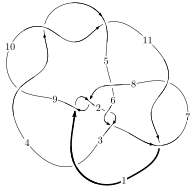
\includegraphics[width=112pt]{../../../GIT/diagram.site/Diagrams/png/595_11a_346.png}\\
\ \ \ A knot diagram\footnotemark}&
\allowdisplaybreaks
\textbf{Linearized knot diagam} \\
\cline{2-2}
 &
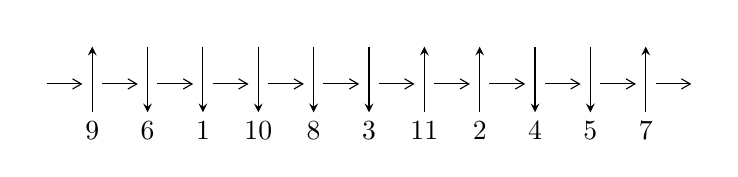
\begin{tikzpicture}[x=20pt, y=17pt]
	% nodes
	\node (C0) at (0, 0) {};
	\node (C1) at (1, 0) {};
	\node (C1U) at (1, +1) {};
	\node (C1D) at (1, -1) {9};

	\node (C2) at (2, 0) {};
	\node (C2U) at (2, +1) {};
	\node (C2D) at (2, -1) {6};

	\node (C3) at (3, 0) {};
	\node (C3U) at (3, +1) {};
	\node (C3D) at (3, -1) {1};

	\node (C4) at (4, 0) {};
	\node (C4U) at (4, +1) {};
	\node (C4D) at (4, -1) {10};

	\node (C5) at (5, 0) {};
	\node (C5U) at (5, +1) {};
	\node (C5D) at (5, -1) {8};

	\node (C6) at (6, 0) {};
	\node (C6U) at (6, +1) {};
	\node (C6D) at (6, -1) {3};

	\node (C7) at (7, 0) {};
	\node (C7U) at (7, +1) {};
	\node (C7D) at (7, -1) {11};

	\node (C8) at (8, 0) {};
	\node (C8U) at (8, +1) {};
	\node (C8D) at (8, -1) {2};

	\node (C9) at (9, 0) {};
	\node (C9U) at (9, +1) {};
	\node (C9D) at (9, -1) {4};

	\node (C10) at (10, 0) {};
	\node (C10U) at (10, +1) {};
	\node (C10D) at (10, -1) {5};

	\node (C11) at (11, 0) {};
	\node (C11U) at (11, +1) {};
	\node (C11D) at (11, -1) {7};
	\node (C12) at (12, 0) {};

	% arrows
	\draw[->,>={angle 60}]
	(C0) edge (C1) (C1) edge (C2) (C2) edge (C3) (C3) edge (C4) (C4) edge (C5) (C5) edge (C6) (C6) edge (C7) (C7) edge (C8) (C8) edge (C9) (C9) edge (C10) (C10) edge (C11) (C11) edge (C12) ;	\draw[->,>=stealth]
	(C1D) edge (C1U) (C2U) edge (C2D) (C3U) edge (C3D) (C4U) edge (C4D) (C5U) edge (C5D) (C6U) edge (C6D) (C7D) edge (C7U) (C8D) edge (C8U) (C9U) edge (C9D) (C10U) edge (C10D) (C11D) edge (C11U) ;
	\end{tikzpicture} \\
\hhline{~~} \\& 
\textbf{Solving Sequence} \\ \cline{2-2} 
 &
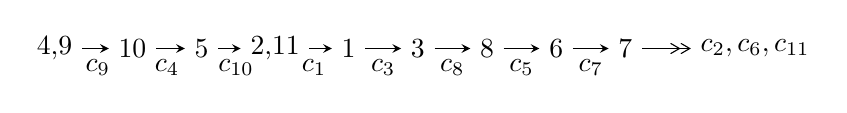
\begin{tikzpicture}[x=25pt, y=7pt]
	% node
	\node (A0) at (-1/8, 0) {4,9};
	\node (A1) at (1, 0) {10};
	\node (A2) at (2, 0) {5};
	\node (A3) at (49/16, 0) {2,11};
	\node (A4) at (33/8, 0) {1};
	\node (A5) at (41/8, 0) {3};
	\node (A6) at (49/8, 0) {8};
	\node (A7) at (57/8, 0) {6};
	\node (A8) at (65/8, 0) {7};
	\node (C1) at (1/2, -1) {$c_{9}$};
	\node (C2) at (3/2, -1) {$c_{4}$};
	\node (C3) at (5/2, -1) {$c_{10}$};
	\node (C4) at (29/8, -1) {$c_{1}$};
	\node (C5) at (37/8, -1) {$c_{3}$};
	\node (C6) at (45/8, -1) {$c_{8}$};
	\node (C7) at (53/8, -1) {$c_{5}$};
	\node (C8) at (61/8, -1) {$c_{7}$};
	\node (A9) at (10, 0) {$c_{2},c_{6},c_{11}$};

	% edge
	\draw[->,>=stealth]	
	(A0) edge (A1) (A1) edge (A2) (A2) edge (A3) (A3) edge (A4) (A4) edge (A5) (A5) edge (A6) (A6) edge (A7) (A7) edge (A8) ;
	\draw[->>,>={angle 60}]	
	(A8) edge (A9);
\end{tikzpicture} \\ 

\end{tabular} \\

\footnotetext{
The image of knot diagram is generated by the software ``\textbf{Draw programme}" developed by Andrew Bartholomew(\url{http://www.layer8.co.uk/maths/draw/index.htm\#Running-draw}), where we modified some parts for our purpose(\url{https://github.com/CATsTAILs/LinksPainter}).
}\phantom \\ \newline 
\centering \textbf{Ideals for irreducible components\footnotemark of $X_{\text{par}}$} 
 
\begin{align*}
I^u_{1}&=\langle 
1008847383871263 u^{22}-3396732854999791 u^{21}+\cdots+181088774400128 b+21567640743990884,\\
\phantom{I^u_{1}}&\phantom{= \langle  }6.16209\times10^{15} u^{22}-2.06878\times10^{16} u^{21}+\cdots+1.44871\times10^{15} a+1.32864\times10^{17},\;u^{23}-3 u^{22}+\cdots+32 u+8\rangle \\
I^u_{2}&=\langle 
-3 u^{14} a+3 u^{14}+\cdots-4 a+11,\;4 u^{13} a-10 u^{14}+\cdots-7 a+9,\\
\phantom{I^u_{2}}&\phantom{= \langle  }u^{15}+u^{14}-8 u^{13}-7 u^{12}+24 u^{11}+16 u^{10}-34 u^9-11 u^8+26 u^7-2 u^6-14 u^5+4 u^3-2 u^2-2 u+1\rangle \\
I^u_{3}&=\langle 
- u^3+b,\;-2 u^3- u^2+3 a-2 u+2,\;u^4- u^2+1\rangle \\
I^u_{4}&=\langle 
b-1,\;4 a- u-2,\;u^2-2\rangle \\
\\
I^v_{1}&=\langle 
a,\;b+1,\;2 v-1\rangle \\
\end{align*}
\raggedright * 5 irreducible components of $\dim_{\mathbb{C}}=0$, with total 60 representations.\\
\footnotetext{All coefficients of polynomials are rational numbers. But the coefficients are sometimes approximated in decimal forms when there is not enough margin.}
\newpage
\renewcommand{\arraystretch}{1}
\centering \section*{I. $I^u_{1}= \langle 1.01\times10^{15} u^{22}-3.40\times10^{15} u^{21}+\cdots+1.81\times10^{14} b+2.16\times10^{16},\;6.16\times10^{15} u^{22}-2.07\times10^{16} u^{21}+\cdots+1.45\times10^{15} a+1.33\times10^{17},\;u^{23}-3 u^{22}+\cdots+32 u+8 \rangle$}
\flushleft \textbf{(i) Arc colorings}\\
\begin{tabular}{m{7pt} m{180pt} m{7pt} m{180pt} }
\flushright $a_{4}=$&$\begin{pmatrix}0\\u\end{pmatrix}$ \\
\flushright $a_{9}=$&$\begin{pmatrix}1\\0\end{pmatrix}$ \\
\flushright $a_{10}=$&$\begin{pmatrix}1\\u^2\end{pmatrix}$ \\
\flushright $a_{5}=$&$\begin{pmatrix}- u\\- u^3+u\end{pmatrix}$ \\
\flushright $a_{2}=$&$\begin{pmatrix}-4.25350 u^{22}+14.2802 u^{21}+\cdots-118.218 u-91.7123\\-5.57101 u^{22}+18.7573 u^{21}+\cdots-156.448 u-119.100\end{pmatrix}$ \\
\flushright $a_{11}=$&$\begin{pmatrix}- u^2+1\\- u^4+2 u^2\end{pmatrix}$ \\
\flushright $a_{1}=$&$\begin{pmatrix}1.31751 u^{22}-4.47711 u^{21}+\cdots+38.2301 u+27.3876\\-5.57101 u^{22}+18.7573 u^{21}+\cdots-156.448 u-119.100\end{pmatrix}$ \\
\flushright $a_{3}=$&$\begin{pmatrix}1.61065 u^{22}-5.45740 u^{21}+\cdots+46.8384 u+34.3216\\-3.62502 u^{22}+12.1065 u^{21}+\cdots-98.5783 u-76.1785\end{pmatrix}$ \\
\flushright $a_{8}=$&$\begin{pmatrix}4.41830 u^{22}-14.8886 u^{21}+\cdots+124.465 u+95.9089\\-5.10401 u^{22}+17.3034 u^{21}+\cdots-145.763 u-110.227\end{pmatrix}$ \\
\flushright $a_{6}=$&$\begin{pmatrix}2.20822 u^{22}-7.37326 u^{21}+\cdots+58.8694 u+46.8606\\-3.43785 u^{22}+11.6995 u^{21}+\cdots-99.4184 u-75.1934\end{pmatrix}$ \\
\flushright $a_{7}=$&$\begin{pmatrix}9.17396 u^{22}-30.9875 u^{21}+\cdots+260.065 u+198.655\\-3.69653 u^{22}+12.5177 u^{21}+\cdots-104.337 u-79.2171\end{pmatrix}$\\ \flushright $a_{7}=$&$\begin{pmatrix}9.17396 u^{22}-30.9875 u^{21}+\cdots+260.065 u+198.655\\-3.69653 u^{22}+12.5177 u^{21}+\cdots-104.337 u-79.2171\end{pmatrix}$\\&\end{tabular}
\flushleft \textbf{(ii) Obstruction class $= -1$}\\~\\
\flushleft \textbf{(iii) Cusp Shapes $= \frac{21095773583741443}{724355097600512} u^{22}-\frac{70909832069661843}{724355097600512} u^{21}+\cdots+\frac{291942728421964629}{362177548800256} u+\frac{110222214152642677}{181088774400128}$}\\~\\
\newpage\renewcommand{\arraystretch}{1}
\flushleft \textbf{(iv) u-Polynomials at the component}\newline \\
\begin{tabular}{m{50pt}|m{274pt}}
Crossings & \hspace{64pt}u-Polynomials at each crossing \\
\hline $$\begin{aligned}c_{1},c_{7},c_{8}\\c_{11}\end{aligned}$$&$\begin{aligned}
&u^{23}+u^{22}+\cdots-14 u-1
\end{aligned}$\\
\hline $$\begin{aligned}c_{2},c_{6}\end{aligned}$$&$\begin{aligned}
&u^{23}+2 u^{22}+\cdots+71 u+8
\end{aligned}$\\
\hline $$\begin{aligned}c_{3},c_{5}\end{aligned}$$&$\begin{aligned}
&8(8 u^{23}-20 u^{22}+\cdots- u-1)
\end{aligned}$\\
\hline $$\begin{aligned}c_{4},c_{9},c_{10}\end{aligned}$$&$\begin{aligned}
&u^{23}-3 u^{22}+\cdots+32 u+8
\end{aligned}$\\
\hline
\end{tabular}\\~\\
\newpage\renewcommand{\arraystretch}{1}
\flushleft \textbf{(v) Riley Polynomials at the component}\newline \\
\begin{tabular}{m{50pt}|m{274pt}}
Crossings & \hspace{64pt}Riley Polynomials at each crossing \\
\hline $$\begin{aligned}c_{1},c_{7},c_{8}\\c_{11}\end{aligned}$$&$\begin{aligned}
&y^{23}+19 y^{22}+\cdots+112 y-1
\end{aligned}$\\
\hline $$\begin{aligned}c_{2},c_{6}\end{aligned}$$&$\begin{aligned}
&y^{23}-14 y^{22}+\cdots+5473 y-64
\end{aligned}$\\
\hline $$\begin{aligned}c_{3},c_{5}\end{aligned}$$&$\begin{aligned}
&64(64 y^{23}-1392 y^{22}+\cdots-37 y-1)
\end{aligned}$\\
\hline $$\begin{aligned}c_{4},c_{9},c_{10}\end{aligned}$$&$\begin{aligned}
&y^{23}-23 y^{22}+\cdots+672 y-64
\end{aligned}$\\
\hline
\end{tabular}\\~\\
\newpage\flushleft \textbf{(vi) Complex Volumes and Cusp Shapes}
$$\begin{array}{c|c|c}  
\text{Solutions to }I^u_{1}& \I (\text{vol} + \sqrt{-1}CS) & \text{Cusp shape}\\
 \hline 
\begin{aligned}
u &= \phantom{-}1.047880 + 0.229903 I \\
a &= \phantom{-}0.109158 + 1.230280 I \\
b &= -0.386436 + 0.666877 I\end{aligned}
 & -2.01223 - 3.75776 I & -5.33334 + 8.56871 I \\ \hline\begin{aligned}
u &= \phantom{-}1.047880 - 0.229903 I \\
a &= \phantom{-}0.109158 - 1.230280 I \\
b &= -0.386436 - 0.666877 I\end{aligned}
 & -2.01223 + 3.75776 I & -5.33334 - 8.56871 I \\ \hline\begin{aligned}
u &= -0.692389 + 0.871381 I \\
a &= \phantom{-}0.897014 - 0.766268 I \\
b &= -0.39680 - 1.43332 I\end{aligned}
 & -10.7273 + 10.3813 I & -10.18639 - 6.73732 I \\ \hline\begin{aligned}
u &= -0.692389 - 0.871381 I \\
a &= \phantom{-}0.897014 + 0.766268 I \\
b &= -0.39680 + 1.43332 I\end{aligned}
 & -10.7273 - 10.3813 I & -10.18639 + 6.73732 I \\ \hline\begin{aligned}
u &= -1.102990 + 0.279147 I \\
a &= -0.429797 + 0.902073 I \\
b &= -0.420512 + 0.719649 I\end{aligned}
 & -2.03566 + 0.84759 I & -5.54570 + 1.19524 I \\ \hline\begin{aligned}
u &= -1.102990 - 0.279147 I \\
a &= -0.429797 - 0.902073 I \\
b &= -0.420512 - 0.719649 I\end{aligned}
 & -2.03566 - 0.84759 I & -5.54570 - 1.19524 I \\ \hline\begin{aligned}
u &= -0.541402 + 1.015810 I \\
a &= \phantom{-}0.411809 - 0.360048 I \\
b &= \phantom{-}0.19561 - 1.40284 I\end{aligned}
 & -10.15960 - 4.19504 I & -11.29932 + 2.35235 I \\ \hline\begin{aligned}
u &= -0.541402 - 1.015810 I \\
a &= \phantom{-}0.411809 + 0.360048 I \\
b &= \phantom{-}0.19561 + 1.40284 I\end{aligned}
 & -10.15960 + 4.19504 I & -11.29932 - 2.35235 I \\ \hline\begin{aligned}
u &= \phantom{-}0.730490 + 1.031710 I \\
a &= \phantom{-}0.548976 + 0.681598 I \\
b &= -0.109506 + 1.309220 I\end{aligned}
 & -5.14680 - 3.47388 I & -11.56230 + 3.97702 I \\ \hline\begin{aligned}
u &= \phantom{-}0.730490 - 1.031710 I \\
a &= \phantom{-}0.548976 - 0.681598 I \\
b &= -0.109506 - 1.309220 I\end{aligned}
 & -5.14680 + 3.47388 I & -11.56230 - 3.97702 I\\
 \hline 
 \end{array}$$\newpage$$\begin{array}{c|c|c}  
\text{Solutions to }I^u_{1}& \I (\text{vol} + \sqrt{-1}CS) & \text{Cusp shape}\\
 \hline 
\begin{aligned}
u &= -1.39374\phantom{ +0.000000I} \\
a &= -0.389467\phantom{ +0.000000I} \\
b &= -0.880255\phantom{ +0.000000I}\end{aligned}
 & -3.32968\phantom{ +0.000000I} & -1.46420\phantom{ +0.000000I} \\ \hline\begin{aligned}
u &= \phantom{-}1.39683\phantom{ +0.000000I} \\
a &= \phantom{-}0.773044\phantom{ +0.000000I} \\
b &= -0.0971819\phantom{ +0.000000I}\end{aligned}
 & -6.54656\phantom{ +0.000000I} & -14.0370\phantom{ +0.000000I} \\ \hline\begin{aligned}
u &= \phantom{-}0.050314 + 0.470724 I \\
a &= -0.460344 + 0.114610 I \\
b &= \phantom{-}0.565086 + 0.372468 I\end{aligned}
 & \phantom{-}0.87976 + 1.13203 I & \phantom{-}3.15244 - 4.47998 I \\ \hline\begin{aligned}
u &= \phantom{-}0.050314 - 0.470724 I \\
a &= -0.460344 - 0.114610 I \\
b &= \phantom{-}0.565086 - 0.372468 I\end{aligned}
 & \phantom{-}0.87976 - 1.13203 I & \phantom{-}3.15244 + 4.47998 I \\ \hline\begin{aligned}
u &= \phantom{-}1.53229\phantom{ +0.000000I} \\
a &= -0.978209\phantom{ +0.000000I} \\
b &= -1.69273\phantom{ +0.000000I}\end{aligned}
 & -6.97375\phantom{ +0.000000I} & -13.5440\phantom{ +0.000000I} \\ \hline\begin{aligned}
u &= -0.373071\phantom{ +0.000000I} \\
a &= -0.558791\phantom{ +0.000000I} \\
b &= \phantom{-}1.23682\phantom{ +0.000000I}\end{aligned}
 & -0.342193\phantom{ +0.000000I} & -19.7630\phantom{ +0.000000I} \\ \hline\begin{aligned}
u &= -0.370526\phantom{ +0.000000I} \\
a &= -1.73277\phantom{ +0.000000I} \\
b &= -0.310175\phantom{ +0.000000I}\end{aligned}
 & -1.09471\phantom{ +0.000000I} & -11.6780\phantom{ +0.000000I} \\ \hline\begin{aligned}
u &= \phantom{-}1.61554 + 0.28548 I \\
a &= -0.64560 - 1.80607 I \\
b &= \phantom{-}0.54587 - 1.52621 I\end{aligned}
 & -18.3248 - 14.6898 I & -11.82186 + 6.64707 I \\ \hline\begin{aligned}
u &= \phantom{-}1.61554 - 0.28548 I \\
a &= -0.64560 + 1.80607 I \\
b &= \phantom{-}0.54587 + 1.52621 I\end{aligned}
 & -18.3248 + 14.6898 I & -11.82186 - 6.64707 I \\ \hline\begin{aligned}
u &= -1.66263 + 0.29375 I \\
a &= -0.52389 + 1.66284 I \\
b &= \phantom{-}0.33582 + 1.42592 I\end{aligned}
 & -13.1520 + 8.3676 I & -10.67653 - 4.81997 I\\
 \hline 
 \end{array}$$\newpage$$\begin{array}{c|c|c}  
\text{Solutions to }I^u_{1}& \I (\text{vol} + \sqrt{-1}CS) & \text{Cusp shape}\\
 \hline 
\begin{aligned}
u &= -1.66263 - 0.29375 I \\
a &= -0.52389 - 1.66284 I \\
b &= \phantom{-}0.33582 - 1.42592 I\end{aligned}
 & -13.1520 - 8.3676 I & -10.67653 + 4.81997 I \\ \hline\begin{aligned}
u &= \phantom{-}1.65930 + 0.36622 I \\
a &= -0.58924 - 1.42409 I \\
b &= \phantom{-}0.04263 - 1.48432 I\end{aligned}
 & -17.3595 - 1.0921 I & -13.73412 + 0. I\phantom{ +0.000000I} \\ \hline\begin{aligned}
u &= \phantom{-}1.65930 - 0.36622 I \\
a &= -0.58924 + 1.42409 I \\
b &= \phantom{-}0.04263 + 1.48432 I\end{aligned}
 & -17.3595 + 1.0921 I & -13.73412 + 0. I\phantom{ +0.000000I}\\
 \hline 
 \end{array}$$\newpage\newpage\renewcommand{\arraystretch}{1}
\centering \section*{II. $I^u_{2}= \langle -3 u^{14} a+3 u^{14}+\cdots-4 a+11,\;4 u^{13} a-10 u^{14}+\cdots-7 a+9,\;u^{15}+u^{14}+\cdots-2 u+1 \rangle$}
\flushleft \textbf{(i) Arc colorings}\\
\begin{tabular}{m{7pt} m{180pt} m{7pt} m{180pt} }
\flushright $a_{4}=$&$\begin{pmatrix}0\\u\end{pmatrix}$ \\
\flushright $a_{9}=$&$\begin{pmatrix}1\\0\end{pmatrix}$ \\
\flushright $a_{10}=$&$\begin{pmatrix}1\\u^2\end{pmatrix}$ \\
\flushright $a_{5}=$&$\begin{pmatrix}- u\\- u^3+u\end{pmatrix}$ \\
\flushright $a_{2}=$&$\begin{pmatrix}a\\\frac{3}{7} u^{14} a-\frac{3}{7} u^{14}+\cdots+\frac{4}{7} a-\frac{11}{7}\end{pmatrix}$ \\
\flushright $a_{11}=$&$\begin{pmatrix}- u^2+1\\- u^4+2 u^2\end{pmatrix}$ \\
\flushright $a_{1}=$&$\begin{pmatrix}-\frac{3}{7} u^{14} a+\frac{3}{7} u^{14}+\cdots+\frac{3}{7} a+\frac{11}{7}\\\frac{3}{7} u^{14} a-\frac{3}{7} u^{14}+\cdots+\frac{4}{7} a-\frac{11}{7}\end{pmatrix}$ \\
\flushright $a_{3}=$&$\begin{pmatrix}-2.28571 a u^{14}-2.71429 u^{14}+\cdots+1.28571 a-3.28571\\-\frac{8}{7} u^{14} a-\frac{6}{7} u^{14}+\cdots-\frac{6}{7} a-\frac{22}{7}\end{pmatrix}$ \\
\flushright $a_{8}=$&$\begin{pmatrix}\frac{3}{7} u^{14} a+\frac{25}{7} u^{14}+\cdots+\frac{11}{7} a-\frac{25}{7}\\-\frac{3}{7} u^{14} a+\frac{3}{7} u^{14}+\cdots-\frac{4}{7} a-\frac{3}{7}\end{pmatrix}$ \\
\flushright $a_{6}=$&$\begin{pmatrix}\frac{6}{7} u^{14} a+\frac{43}{7} u^{14}+\cdots+\frac{22}{7} a-\frac{8}{7}\\\frac{12}{7} u^{14} a+\frac{16}{7} u^{14}+\cdots+\frac{9}{7} a-\frac{9}{7}\end{pmatrix}$ \\
\flushright $a_{7}=$&$\begin{pmatrix}\frac{3}{7} u^{14} a+\frac{25}{7} u^{14}+\cdots+\frac{11}{7} a-\frac{32}{7}\\-1\end{pmatrix}$\\ \flushright $a_{7}=$&$\begin{pmatrix}\frac{3}{7} u^{14} a+\frac{25}{7} u^{14}+\cdots+\frac{11}{7} a-\frac{32}{7}\\-1\end{pmatrix}$\\&\end{tabular}
\flushleft \textbf{(ii) Obstruction class $= -1$}\\~\\
\flushleft \textbf{(iii) Cusp Shapes $= 4 u^{13}-32 u^{11}+92 u^9-4 u^8-112 u^7+20 u^6+56 u^5-28 u^4-20 u^3+8 u^2+4 u-14$}\\~\\
\newpage\renewcommand{\arraystretch}{1}
\flushleft \textbf{(iv) u-Polynomials at the component}\newline \\
\begin{tabular}{m{50pt}|m{274pt}}
Crossings & \hspace{64pt}u-Polynomials at each crossing \\
\hline $$\begin{aligned}c_{1},c_{7},c_{8}\\c_{11}\end{aligned}$$&$\begin{aligned}
&u^{30}-3 u^{29}+\cdots+8 u+13
\end{aligned}$\\
\hline $$\begin{aligned}c_{2},c_{6}\end{aligned}$$&$\begin{aligned}
&(u^{15}+u^{14}+\cdots-2 u-1)^{2}
\end{aligned}$\\
\hline $$\begin{aligned}c_{3},c_{5}\end{aligned}$$&$\begin{aligned}
&u^{30}+3 u^{29}+\cdots-67460 u+14279
\end{aligned}$\\
\hline $$\begin{aligned}c_{4},c_{9},c_{10}\end{aligned}$$&$\begin{aligned}
&(u^{15}+u^{14}+\cdots-2 u+1)^{2}
\end{aligned}$\\
\hline
\end{tabular}\\~\\
\newpage\renewcommand{\arraystretch}{1}
\flushleft \textbf{(v) Riley Polynomials at the component}\newline \\
\begin{tabular}{m{50pt}|m{274pt}}
Crossings & \hspace{64pt}Riley Polynomials at each crossing \\
\hline $$\begin{aligned}c_{1},c_{7},c_{8}\\c_{11}\end{aligned}$$&$\begin{aligned}
&y^{30}+23 y^{29}+\cdots-1572 y+169
\end{aligned}$\\
\hline $$\begin{aligned}c_{2},c_{6}\end{aligned}$$&$\begin{aligned}
&(y^{15}-13 y^{14}+\cdots+8 y-1)^{2}
\end{aligned}$\\
\hline $$\begin{aligned}c_{3},c_{5}\end{aligned}$$&$\begin{aligned}
&y^{30}-21 y^{29}+\cdots-2895344340 y+203889841
\end{aligned}$\\
\hline $$\begin{aligned}c_{4},c_{9},c_{10}\end{aligned}$$&$\begin{aligned}
&(y^{15}-17 y^{14}+\cdots+8 y-1)^{2}
\end{aligned}$\\
\hline
\end{tabular}\\~\\
\newpage\flushleft \textbf{(vi) Complex Volumes and Cusp Shapes}
$$\begin{array}{c|c|c}  
\text{Solutions to }I^u_{2}& \I (\text{vol} + \sqrt{-1}CS) & \text{Cusp shape}\\
 \hline 
\begin{aligned}
u &= -0.837202\phantom{ +0.000000I} \\
a &= \phantom{-}0.948699 + 0.418317 I \\
b &= -0.455272 + 1.273510 I\end{aligned}
 & -8.81535\phantom{ +0.000000I} & -13.0390\phantom{ +0.000000I} \\ \hline\begin{aligned}
u &= -0.837202\phantom{ +0.000000I} \\
a &= \phantom{-}0.948699 - 0.418317 I \\
b &= -0.455272 - 1.273510 I\end{aligned}
 & -8.81535\phantom{ +0.000000I} & -13.0390\phantom{ +0.000000I} \\ \hline\begin{aligned}
u &= \phantom{-}0.616241 + 0.538656 I \\
a &= -0.877744 - 0.781079 I \\
b &= \phantom{-}0.37957 - 1.41365 I\end{aligned}
 & -5.47316 - 5.45324 I & -7.99532 + 6.35130 I \\ \hline\begin{aligned}
u &= \phantom{-}0.616241 + 0.538656 I \\
a &= \phantom{-}0.634060 + 0.127928 I \\
b &= -0.991485 + 0.204855 I\end{aligned}
 & -5.47316 - 5.45324 I & -7.99532 + 6.35130 I \\ \hline\begin{aligned}
u &= \phantom{-}0.616241 - 0.538656 I \\
a &= -0.877744 + 0.781079 I \\
b &= \phantom{-}0.37957 + 1.41365 I\end{aligned}
 & -5.47316 + 5.45324 I & -7.99532 - 6.35130 I \\ \hline\begin{aligned}
u &= \phantom{-}0.616241 - 0.538656 I \\
a &= \phantom{-}0.634060 - 0.127928 I \\
b &= -0.991485 - 0.204855 I\end{aligned}
 & -5.47316 + 5.45324 I & -7.99532 - 6.35130 I \\ \hline\begin{aligned}
u &= -0.486836 + 0.521522 I \\
a &= -0.982556 + 0.802109 I \\
b &= \phantom{-}0.186786 + 1.050900 I\end{aligned}
 & -1.11561 + 1.81248 I & -2.14381 - 4.33913 I \\ \hline\begin{aligned}
u &= -0.486836 + 0.521522 I \\
a &= \phantom{-}0.275176 + 0.534678 I \\
b &= -0.373462 + 0.000206 I\end{aligned}
 & -1.11561 + 1.81248 I & -2.14381 - 4.33913 I \\ \hline\begin{aligned}
u &= -0.486836 - 0.521522 I \\
a &= -0.982556 - 0.802109 I \\
b &= \phantom{-}0.186786 - 1.050900 I\end{aligned}
 & -1.11561 - 1.81248 I & -2.14381 + 4.33913 I \\ \hline\begin{aligned}
u &= -0.486836 - 0.521522 I \\
a &= \phantom{-}0.275176 - 0.534678 I \\
b &= -0.373462 - 0.000206 I\end{aligned}
 & -1.11561 - 1.81248 I & -2.14381 + 4.33913 I\\
 \hline 
 \end{array}$$\newpage$$\begin{array}{c|c|c}  
\text{Solutions to }I^u_{2}& \I (\text{vol} + \sqrt{-1}CS) & \text{Cusp shape}\\
 \hline 
\begin{aligned}
u &= \phantom{-}0.309525 + 0.567792 I \\
a &= -1.61115 + 0.22060 I \\
b &= -0.116215 - 1.234430 I\end{aligned}
 & -4.58881 + 1.64925 I & -5.60633 - 0.16522 I \\ \hline\begin{aligned}
u &= \phantom{-}0.309525 + 0.567792 I \\
a &= -0.47283 - 1.80977 I \\
b &= \phantom{-}0.497171 + 0.372159 I\end{aligned}
 & -4.58881 + 1.64925 I & -5.60633 - 0.16522 I \\ \hline\begin{aligned}
u &= \phantom{-}0.309525 - 0.567792 I \\
a &= -1.61115 - 0.22060 I \\
b &= -0.116215 + 1.234430 I\end{aligned}
 & -4.58881 - 1.64925 I & -5.60633 + 0.16522 I \\ \hline\begin{aligned}
u &= \phantom{-}0.309525 - 0.567792 I \\
a &= -0.47283 + 1.80977 I \\
b &= \phantom{-}0.497171 - 0.372159 I\end{aligned}
 & -4.58881 - 1.64925 I & -5.60633 + 0.16522 I \\ \hline\begin{aligned}
u &= -1.48203 + 0.05428 I \\
a &= -1.80599 + 0.58512 I \\
b &= \phantom{-}0.312806 + 0.818632 I\end{aligned}
 & -10.05370 + 0.15908 I & -9.79403 + 0.85194 I \\ \hline\begin{aligned}
u &= -1.48203 + 0.05428 I \\
a &= \phantom{-}0.39717 - 3.25376 I \\
b &= \phantom{-}0.085684 - 1.202650 I\end{aligned}
 & -10.05370 + 0.15908 I & -9.79403 + 0.85194 I \\ \hline\begin{aligned}
u &= -1.48203 - 0.05428 I \\
a &= -1.80599 - 0.58512 I \\
b &= \phantom{-}0.312806 - 0.818632 I\end{aligned}
 & -10.05370 - 0.15908 I & -9.79403 - 0.85194 I \\ \hline\begin{aligned}
u &= -1.48203 - 0.05428 I \\
a &= \phantom{-}0.39717 + 3.25376 I \\
b &= \phantom{-}0.085684 + 1.202650 I\end{aligned}
 & -10.05370 - 0.15908 I & -9.79403 - 0.85194 I \\ \hline\begin{aligned}
u &= \phantom{-}1.52656 + 0.13829 I \\
a &= \phantom{-}0.104118 - 0.130246 I \\
b &= \phantom{-}0.839538 - 0.236157 I\end{aligned}
 & -7.81260 - 4.11725 I & -6.59688 + 3.71929 I \\ \hline\begin{aligned}
u &= \phantom{-}1.52656 + 0.13829 I \\
a &= \phantom{-}0.49462 + 2.01049 I \\
b &= -0.298420 + 1.343440 I\end{aligned}
 & -7.81260 - 4.11725 I & -6.59688 + 3.71929 I\\
 \hline 
 \end{array}$$\newpage$$\begin{array}{c|c|c}  
\text{Solutions to }I^u_{2}& \I (\text{vol} + \sqrt{-1}CS) & \text{Cusp shape}\\
 \hline 
\begin{aligned}
u &= \phantom{-}1.52656 - 0.13829 I \\
a &= \phantom{-}0.104118 + 0.130246 I \\
b &= \phantom{-}0.839538 + 0.236157 I\end{aligned}
 & -7.81260 + 4.11725 I & -6.59688 - 3.71929 I \\ \hline\begin{aligned}
u &= \phantom{-}1.52656 - 0.13829 I \\
a &= \phantom{-}0.49462 - 2.01049 I \\
b &= -0.298420 - 1.343440 I\end{aligned}
 & -7.81260 + 4.11725 I & -6.59688 - 3.71929 I \\ \hline\begin{aligned}
u &= -1.57098 + 0.16034 I \\
a &= \phantom{-}0.532723 + 0.450416 I \\
b &= \phantom{-}1.381210 + 0.203773 I\end{aligned}
 & -12.8088 + 8.0168 I & -11.04132 - 4.89679 I \\ \hline\begin{aligned}
u &= -1.57098 + 0.16034 I \\
a &= \phantom{-}0.31812 - 1.99419 I \\
b &= -0.55486 - 1.65691 I\end{aligned}
 & -12.8088 + 8.0168 I & -11.04132 - 4.89679 I \\ \hline\begin{aligned}
u &= -1.57098 - 0.16034 I \\
a &= \phantom{-}0.532723 - 0.450416 I \\
b &= \phantom{-}1.381210 - 0.203773 I\end{aligned}
 & -12.8088 - 8.0168 I & -11.04132 + 4.89679 I \\ \hline\begin{aligned}
u &= -1.57098 - 0.16034 I \\
a &= \phantom{-}0.31812 + 1.99419 I \\
b &= -0.55486 + 1.65691 I\end{aligned}
 & -12.8088 - 8.0168 I & -11.04132 + 4.89679 I \\ \hline\begin{aligned}
u &= \phantom{-}0.404272\phantom{ +0.000000I} \\
a &= \phantom{-}2.91327 + 2.87968 I \\
b &= -0.150080 + 1.033230 I\end{aligned}
 & -3.88780\phantom{ +0.000000I} & -12.6280\phantom{ +0.000000I} \\ \hline\begin{aligned}
u &= \phantom{-}0.404272\phantom{ +0.000000I} \\
a &= \phantom{-}2.91327 - 2.87968 I \\
b &= -0.150080 - 1.033230 I\end{aligned}
 & -3.88780\phantom{ +0.000000I} & -12.6280\phantom{ +0.000000I} \\ \hline\begin{aligned}
u &= \phantom{-}1.60797\phantom{ +0.000000I} \\
a &= \phantom{-}0.13231 + 1.72692 I \\
b &= \phantom{-}0.75703 + 1.64902 I\end{aligned}
 & -17.0919\phantom{ +0.000000I} & -13.9770\phantom{ +0.000000I} \\ \hline\begin{aligned}
u &= \phantom{-}1.60797\phantom{ +0.000000I} \\
a &= \phantom{-}0.13231 - 1.72692 I \\
b &= \phantom{-}0.75703 - 1.64902 I\end{aligned}
 & -17.0919\phantom{ +0.000000I} & -13.9770\phantom{ +0.000000I}\\
 \hline 
 \end{array}$$\newpage\newpage\renewcommand{\arraystretch}{1}
\centering \section*{III. $I^u_{3}= \langle - u^3+b,\;-2 u^3- u^2+3 a-2 u+2,\;u^4- u^2+1 \rangle$}
\flushleft \textbf{(i) Arc colorings}\\
\begin{tabular}{m{7pt} m{180pt} m{7pt} m{180pt} }
\flushright $a_{4}=$&$\begin{pmatrix}0\\u\end{pmatrix}$ \\
\flushright $a_{9}=$&$\begin{pmatrix}1\\0\end{pmatrix}$ \\
\flushright $a_{10}=$&$\begin{pmatrix}1\\u^2\end{pmatrix}$ \\
\flushright $a_{5}=$&$\begin{pmatrix}- u\\- u^3+u\end{pmatrix}$ \\
\flushright $a_{2}=$&$\begin{pmatrix}\frac{2}{3} u^3+\frac{1}{3} u^2+\frac{2}{3} u-\frac{2}{3}\\u^3\end{pmatrix}$ \\
\flushright $a_{11}=$&$\begin{pmatrix}- u^2+1\\u^2+1\end{pmatrix}$ \\
\flushright $a_{1}=$&$\begin{pmatrix}-\frac{1}{3} u^3+\frac{1}{3} u^2+\frac{2}{3} u-\frac{2}{3}\\u^3\end{pmatrix}$ \\
\flushright $a_{3}=$&$\begin{pmatrix}-\frac{1}{3} u^3+\frac{2}{3} u-\frac{2}{3}\\\frac{2}{3} u^3-\frac{2}{3} u^2+\frac{2}{3} u+\frac{1}{3}\end{pmatrix}$ \\
\flushright $a_{8}=$&$\begin{pmatrix}-\frac{1}{3} u^3+\frac{2}{3} u^2-\frac{1}{3} u-\frac{1}{3}\\-1\end{pmatrix}$ \\
\flushright $a_{6}=$&$\begin{pmatrix}- u-\frac{1}{3}\\-\frac{2}{3} u^3-\frac{1}{3} u^2+\frac{1}{3} u-\frac{1}{3}\end{pmatrix}$ \\
\flushright $a_{7}=$&$\begin{pmatrix}-\frac{1}{3} u^3+\frac{2}{3} u^2-\frac{4}{3} u-\frac{1}{3}\\-2 u^3+u-1\end{pmatrix}$\\ \flushright $a_{7}=$&$\begin{pmatrix}-\frac{1}{3} u^3+\frac{2}{3} u^2-\frac{4}{3} u-\frac{1}{3}\\-2 u^3+u-1\end{pmatrix}$\\&\end{tabular}
\flushleft \textbf{(ii) Obstruction class $= 1$}\\~\\
\flushleft \textbf{(iii) Cusp Shapes $= 4 u^2-12$}\\~\\
\newpage\renewcommand{\arraystretch}{1}
\flushleft \textbf{(iv) u-Polynomials at the component}\newline \\
\begin{tabular}{m{50pt}|m{274pt}}
Crossings & \hspace{64pt}u-Polynomials at each crossing \\
\hline $$\begin{aligned}c_{1},c_{7},c_{8}\\c_{11}\end{aligned}$$&$\begin{aligned}
&(u^2+1)^2
\end{aligned}$\\
\hline $$\begin{aligned}c_{2}\end{aligned}$$&$\begin{aligned}
&(u^2- u+1)^2
\end{aligned}$\\
\hline $$\begin{aligned}c_{3}\end{aligned}$$&$\begin{aligned}
&9(9 u^4+18 u^3+9 u^2+1)
\end{aligned}$\\
\hline $$\begin{aligned}c_{4},c_{9},c_{10}\end{aligned}$$&$\begin{aligned}
&u^4- u^2+1
\end{aligned}$\\
\hline $$\begin{aligned}c_{5}\end{aligned}$$&$\begin{aligned}
&9(9 u^4-18 u^3+9 u^2+1)
\end{aligned}$\\
\hline $$\begin{aligned}c_{6}\end{aligned}$$&$\begin{aligned}
&(u^2+u+1)^2
\end{aligned}$\\
\hline
\end{tabular}\\~\\
\newpage\renewcommand{\arraystretch}{1}
\flushleft \textbf{(v) Riley Polynomials at the component}\newline \\
\begin{tabular}{m{50pt}|m{274pt}}
Crossings & \hspace{64pt}Riley Polynomials at each crossing \\
\hline $$\begin{aligned}c_{1},c_{7},c_{8}\\c_{11}\end{aligned}$$&$\begin{aligned}
&(y+1)^4
\end{aligned}$\\
\hline $$\begin{aligned}c_{2},c_{6}\end{aligned}$$&$\begin{aligned}
&(y^2+y+1)^2
\end{aligned}$\\
\hline $$\begin{aligned}c_{3},c_{5}\end{aligned}$$&$\begin{aligned}
&81(81 y^4-162 y^3+99 y^2+18 y+1)
\end{aligned}$\\
\hline $$\begin{aligned}c_{4},c_{9},c_{10}\end{aligned}$$&$\begin{aligned}
&(y^2- y+1)^2
\end{aligned}$\\
\hline
\end{tabular}\\~\\
\newpage\flushleft \textbf{(vi) Complex Volumes and Cusp Shapes}
$$\begin{array}{c|c|c}  
\text{Solutions to }I^u_{3}& \I (\text{vol} + \sqrt{-1}CS) & \text{Cusp shape}\\
 \hline 
\begin{aligned}
u &= \phantom{-}0.866025 + 0.500000 I \\
a &= \phantom{-}0.077350 + 1.288680 I \\
b &= \phantom{-0.000000 -}1.000000 I\end{aligned}
 & -3.28987 - 2.02988 I & -10.00000 + 3.46410 I \\ \hline\begin{aligned}
u &= \phantom{-}0.866025 - 0.500000 I \\
a &= \phantom{-}0.077350 - 1.288680 I \\
b &= \phantom{-0.000000 } -1.000000 I\end{aligned}
 & -3.28987 + 2.02988 I & -10.00000 - 3.46410 I \\ \hline\begin{aligned}
u &= -0.866025 + 0.500000 I \\
a &= -1.077350 + 0.711325 I \\
b &= \phantom{-0.000000 -}1.000000 I\end{aligned}
 & -3.28987 + 2.02988 I & -10.00000 - 3.46410 I \\ \hline\begin{aligned}
u &= -0.866025 - 0.500000 I \\
a &= -1.077350 - 0.711325 I \\
b &= \phantom{-0.000000 } -1.000000 I\end{aligned}
 & -3.28987 - 2.02988 I & -10.00000 + 3.46410 I\\
 \hline 
 \end{array}$$\newpage\newpage\renewcommand{\arraystretch}{1}
\centering \section*{IV. $I^u_{4}= \langle b-1,\;4 a- u-2,\;u^2-2 \rangle$}
\flushleft \textbf{(i) Arc colorings}\\
\begin{tabular}{m{7pt} m{180pt} m{7pt} m{180pt} }
\flushright $a_{4}=$&$\begin{pmatrix}0\\u\end{pmatrix}$ \\
\flushright $a_{9}=$&$\begin{pmatrix}1\\0\end{pmatrix}$ \\
\flushright $a_{10}=$&$\begin{pmatrix}1\\2\end{pmatrix}$ \\
\flushright $a_{5}=$&$\begin{pmatrix}- u\\- u\end{pmatrix}$ \\
\flushright $a_{2}=$&$\begin{pmatrix}\frac{1}{4} u+\frac{1}{2}\\1\end{pmatrix}$ \\
\flushright $a_{11}=$&$\begin{pmatrix}-1\\0\end{pmatrix}$ \\
\flushright $a_{1}=$&$\begin{pmatrix}\frac{1}{4} u-\frac{1}{2}\\1\end{pmatrix}$ \\
\flushright $a_{3}=$&$\begin{pmatrix}\frac{3}{8} u-\frac{1}{2}\\\frac{1}{2} u+\frac{1}{2}\end{pmatrix}$ \\
\flushright $a_{8}=$&$\begin{pmatrix}\frac{1}{4} u+\frac{3}{2}\\1\end{pmatrix}$ \\
\flushright $a_{6}=$&$\begin{pmatrix}-\frac{1}{8} u+1\\-\frac{1}{2} u+\frac{1}{2}\end{pmatrix}$ \\
\flushright $a_{7}=$&$\begin{pmatrix}\frac{1}{4} u+\frac{1}{2}\\1\end{pmatrix}$\\ \flushright $a_{7}=$&$\begin{pmatrix}\frac{1}{4} u+\frac{1}{2}\\1\end{pmatrix}$\\&\end{tabular}
\flushleft \textbf{(ii) Obstruction class $= 1$}\\~\\
\flushleft \textbf{(iii) Cusp Shapes $= -8$}\\~\\
\newpage\renewcommand{\arraystretch}{1}
\flushleft \textbf{(iv) u-Polynomials at the component}\newline \\
\begin{tabular}{m{50pt}|m{274pt}}
Crossings & \hspace{64pt}u-Polynomials at each crossing \\
\hline $$\begin{aligned}c_{1},c_{2},c_{11}\end{aligned}$$&$\begin{aligned}
&(u+1)^2
\end{aligned}$\\
\hline $$\begin{aligned}c_{3}\end{aligned}$$&$\begin{aligned}
&4(4 u^2+4 u-1)
\end{aligned}$\\
\hline $$\begin{aligned}c_{4},c_{9},c_{10}\end{aligned}$$&$\begin{aligned}
&u^2-2
\end{aligned}$\\
\hline $$\begin{aligned}c_{5}\end{aligned}$$&$\begin{aligned}
&4(4 u^2-4 u-1)
\end{aligned}$\\
\hline $$\begin{aligned}c_{6},c_{7},c_{8}\end{aligned}$$&$\begin{aligned}
&(u-1)^2
\end{aligned}$\\
\hline
\end{tabular}\\~\\
\newpage\renewcommand{\arraystretch}{1}
\flushleft \textbf{(v) Riley Polynomials at the component}\newline \\
\begin{tabular}{m{50pt}|m{274pt}}
Crossings & \hspace{64pt}Riley Polynomials at each crossing \\
\hline $$\begin{aligned}c_{1},c_{2},c_{6}\\c_{7},c_{8},c_{11}\end{aligned}$$&$\begin{aligned}
&(y-1)^2
\end{aligned}$\\
\hline $$\begin{aligned}c_{3},c_{5}\end{aligned}$$&$\begin{aligned}
&16(16 y^2-24 y+1)
\end{aligned}$\\
\hline $$\begin{aligned}c_{4},c_{9},c_{10}\end{aligned}$$&$\begin{aligned}
&(y-2)^2
\end{aligned}$\\
\hline
\end{tabular}\\~\\
\newpage\flushleft \textbf{(vi) Complex Volumes and Cusp Shapes}
$$\begin{array}{c|c|c}  
\text{Solutions to }I^u_{4}& \I (\text{vol} + \sqrt{-1}CS) & \text{Cusp shape}\\
 \hline 
\begin{aligned}
u &= \phantom{-}1.41421\phantom{ +0.000000I} \\
a &= \phantom{-}0.853553\phantom{ +0.000000I} \\
b &= \phantom{-}1.00000\phantom{ +0.000000I}\end{aligned}
 & -4.93480\phantom{ +0.000000I} & -8.00000\phantom{ +0.000000I} \\ \hline\begin{aligned}
u &= -1.41421\phantom{ +0.000000I} \\
a &= \phantom{-}0.146447\phantom{ +0.000000I} \\
b &= \phantom{-}1.00000\phantom{ +0.000000I}\end{aligned}
 & -4.93480\phantom{ +0.000000I} & -8.00000\phantom{ +0.000000I}\\
 \hline 
 \end{array}$$\newpage\newpage\renewcommand{\arraystretch}{1}
\centering \section*{V. $I^v_{1}= \langle a,\;b+1,\;2 v-1 \rangle$}
\flushleft \textbf{(i) Arc colorings}\\
\begin{tabular}{m{7pt} m{180pt} m{7pt} m{180pt} }
\flushright $a_{4}=$&$\begin{pmatrix}0.5\\0\end{pmatrix}$ \\
\flushright $a_{9}=$&$\begin{pmatrix}1\\0\end{pmatrix}$ \\
\flushright $a_{10}=$&$\begin{pmatrix}1\\0\end{pmatrix}$ \\
\flushright $a_{5}=$&$\begin{pmatrix}0.5\\0\end{pmatrix}$ \\
\flushright $a_{2}=$&$\begin{pmatrix}0\\-1\end{pmatrix}$ \\
\flushright $a_{11}=$&$\begin{pmatrix}1\\0\end{pmatrix}$ \\
\flushright $a_{1}=$&$\begin{pmatrix}1\\-1\end{pmatrix}$ \\
\flushright $a_{3}=$&$\begin{pmatrix}1\\-0.5\end{pmatrix}$ \\
\flushright $a_{8}=$&$\begin{pmatrix}1\\1\end{pmatrix}$ \\
\flushright $a_{6}=$&$\begin{pmatrix}1\\0.5\end{pmatrix}$ \\
\flushright $a_{7}=$&$\begin{pmatrix}0\\1\end{pmatrix}$\\ \flushright $a_{7}=$&$\begin{pmatrix}0\\1\end{pmatrix}$\\&\end{tabular}
\flushleft \textbf{(ii) Obstruction class $= 1$}\\~\\
\flushleft \textbf{(iii) Cusp Shapes $= 4.5$}\\~\\
\newpage\renewcommand{\arraystretch}{1}
\flushleft \textbf{(iv) u-Polynomials at the component}\newline \\
\begin{tabular}{m{50pt}|m{274pt}}
Crossings & \hspace{64pt}u-Polynomials at each crossing \\
\hline $$\begin{aligned}c_{1},c_{2},c_{11}\end{aligned}$$&$\begin{aligned}
&u-1
\end{aligned}$\\
\hline $$\begin{aligned}c_{3}\end{aligned}$$&$\begin{aligned}
&2(2 u+1)
\end{aligned}$\\
\hline $$\begin{aligned}c_{4},c_{9},c_{10}\end{aligned}$$&$\begin{aligned}
&u
\end{aligned}$\\
\hline $$\begin{aligned}c_{5}\end{aligned}$$&$\begin{aligned}
&2(2 u-1)
\end{aligned}$\\
\hline $$\begin{aligned}c_{6},c_{7},c_{8}\end{aligned}$$&$\begin{aligned}
&u+1
\end{aligned}$\\
\hline
\end{tabular}\\~\\
\newpage\renewcommand{\arraystretch}{1}
\flushleft \textbf{(v) Riley Polynomials at the component}\newline \\
\begin{tabular}{m{50pt}|m{274pt}}
Crossings & \hspace{64pt}Riley Polynomials at each crossing \\
\hline $$\begin{aligned}c_{1},c_{2},c_{6}\\c_{7},c_{8},c_{11}\end{aligned}$$&$\begin{aligned}
&y-1
\end{aligned}$\\
\hline $$\begin{aligned}c_{3},c_{5}\end{aligned}$$&$\begin{aligned}
&4(4 y-1)
\end{aligned}$\\
\hline $$\begin{aligned}c_{4},c_{9},c_{10}\end{aligned}$$&$\begin{aligned}
&y
\end{aligned}$\\
\hline
\end{tabular}\\~\\
\newpage\flushleft \textbf{(vi) Complex Volumes and Cusp Shapes}
$$\begin{array}{c|c|c}  
\text{Solutions to }I^v_{1}& \I (\text{vol} + \sqrt{-1}CS) & \text{Cusp shape}\\
 \hline 
\begin{aligned}
v &= \phantom{-}0.500000\phantom{ +0.000000I} \\
a &= \phantom{-0.000000 } 0 \\
b &= -1.00000\phantom{ +0.000000I}\end{aligned}
 & \phantom{-0.000000 } 0 & \phantom{-}4.50000\phantom{ +0.000000I}\\
 \hline 
 \end{array}$$\newpage
\newpage\renewcommand{\arraystretch}{1}
\centering \section*{ VI. u-Polynomials}
\begin{tabular}{m{50pt}|m{274pt}}
Crossings & \hspace{64pt}u-Polynomials at each crossing \\
\hline $$\begin{aligned}c_{1},c_{11}\end{aligned}$$&$\begin{aligned}
&(u-1)(u+1)^2(u^2+1)^2(u^{23}+u^{22}+\cdots-14 u-1)\\
&\cdot(u^{30}-3 u^{29}+\cdots+8 u+13)
\end{aligned}$\\
\hline $$\begin{aligned}c_{2}\end{aligned}$$&$\begin{aligned}
&(u-1)(u+1)^2(u^2- u+1)^2(u^{15}+u^{14}+\cdots-2 u-1)^{2}\\
&\cdot(u^{23}+2 u^{22}+\cdots+71 u+8)
\end{aligned}$\\
\hline $$\begin{aligned}c_{3}\end{aligned}$$&$\begin{aligned}
&576(2 u+1)(4 u^2+4 u-1)(9 u^4+18 u^3+9 u^2+1)\\
&\cdot(8 u^{23}-20 u^{22}+\cdots- u-1)(u^{30}+3 u^{29}+\cdots-67460 u+14279)
\end{aligned}$\\
\hline $$\begin{aligned}c_{4},c_{9},c_{10}\end{aligned}$$&$\begin{aligned}
&u(u^2-2)(u^4- u^2+1)(u^{15}+u^{14}+\cdots-2 u+1)^{2}\\
&\cdot(u^{23}-3 u^{22}+\cdots+32 u+8)
\end{aligned}$\\
\hline $$\begin{aligned}c_{5}\end{aligned}$$&$\begin{aligned}
&576(2 u-1)(4 u^2-4 u-1)(9 u^4-18 u^3+9 u^2+1)\\
&\cdot(8 u^{23}-20 u^{22}+\cdots- u-1)(u^{30}+3 u^{29}+\cdots-67460 u+14279)
\end{aligned}$\\
\hline $$\begin{aligned}c_{6}\end{aligned}$$&$\begin{aligned}
&((u-1)^2)(u+1)(u^2+u+1)^2(u^{15}+u^{14}+\cdots-2 u-1)^{2}\\
&\cdot(u^{23}+2 u^{22}+\cdots+71 u+8)
\end{aligned}$\\
\hline $$\begin{aligned}c_{7},c_{8}\end{aligned}$$&$\begin{aligned}
&((u-1)^2)(u+1)(u^2+1)^2(u^{23}+u^{22}+\cdots-14 u-1)\\
&\cdot(u^{30}-3 u^{29}+\cdots+8 u+13)
\end{aligned}$\\
\hline
\end{tabular}\newpage\renewcommand{\arraystretch}{1}
\centering \section*{ VII. Riley Polynomials}
\begin{tabular}{m{50pt}|m{274pt}}
Crossings & \hspace{64pt}Riley Polynomials at each crossing \\
\hline $$\begin{aligned}c_{1},c_{7},c_{8}\\c_{11}\end{aligned}$$&$\begin{aligned}
&((y-1)^3)(y+1)^4(y^{23}+19 y^{22}+\cdots+112 y-1)\\
&\cdot(y^{30}+23 y^{29}+\cdots-1572 y+169)
\end{aligned}$\\
\hline $$\begin{aligned}c_{2},c_{6}\end{aligned}$$&$\begin{aligned}
&((y-1)^3)(y^2+y+1)^2(y^{15}-13 y^{14}+\cdots+8 y-1)^{2}\\
&\cdot(y^{23}-14 y^{22}+\cdots+5473 y-64)
\end{aligned}$\\
\hline $$\begin{aligned}c_{3},c_{5}\end{aligned}$$&$\begin{aligned}
&331776(4 y-1)(16 y^2-24 y+1)(81 y^{4}-162 y^{3}+\cdots+18 y+1)\\
&\cdot(64 y^{23}-1392 y^{22}+\cdots-37 y-1)\\
&\cdot(y^{30}-21 y^{29}+\cdots-2895344340 y+203889841)
\end{aligned}$\\
\hline $$\begin{aligned}c_{4},c_{9},c_{10}\end{aligned}$$&$\begin{aligned}
&y(y-2)^2(y^2- y+1)^2(y^{15}-17 y^{14}+\cdots+8 y-1)^{2}\\
&\cdot(y^{23}-23 y^{22}+\cdots+672 y-64)
\end{aligned}$\\
\hline
\end{tabular}
\vskip 2pc
\end{document}